\section{System Model and Problem Formulation}
\label{sec:system}

\subsection{Scenario}
We consider one LEO/NTN edge node equipped with a sensor-facing task queue, a constrained accelerator, and an intermittent downlink. As shown in \Cref{fig:arch}, tasks enter an on-board queue. A replaceable LLM profile supplies energy, latency, and memory costs; an orbital contact schedule supplies ground-station windows; the scheduler selects an action for each task.

\begin{figure}[tb]
  \centering
  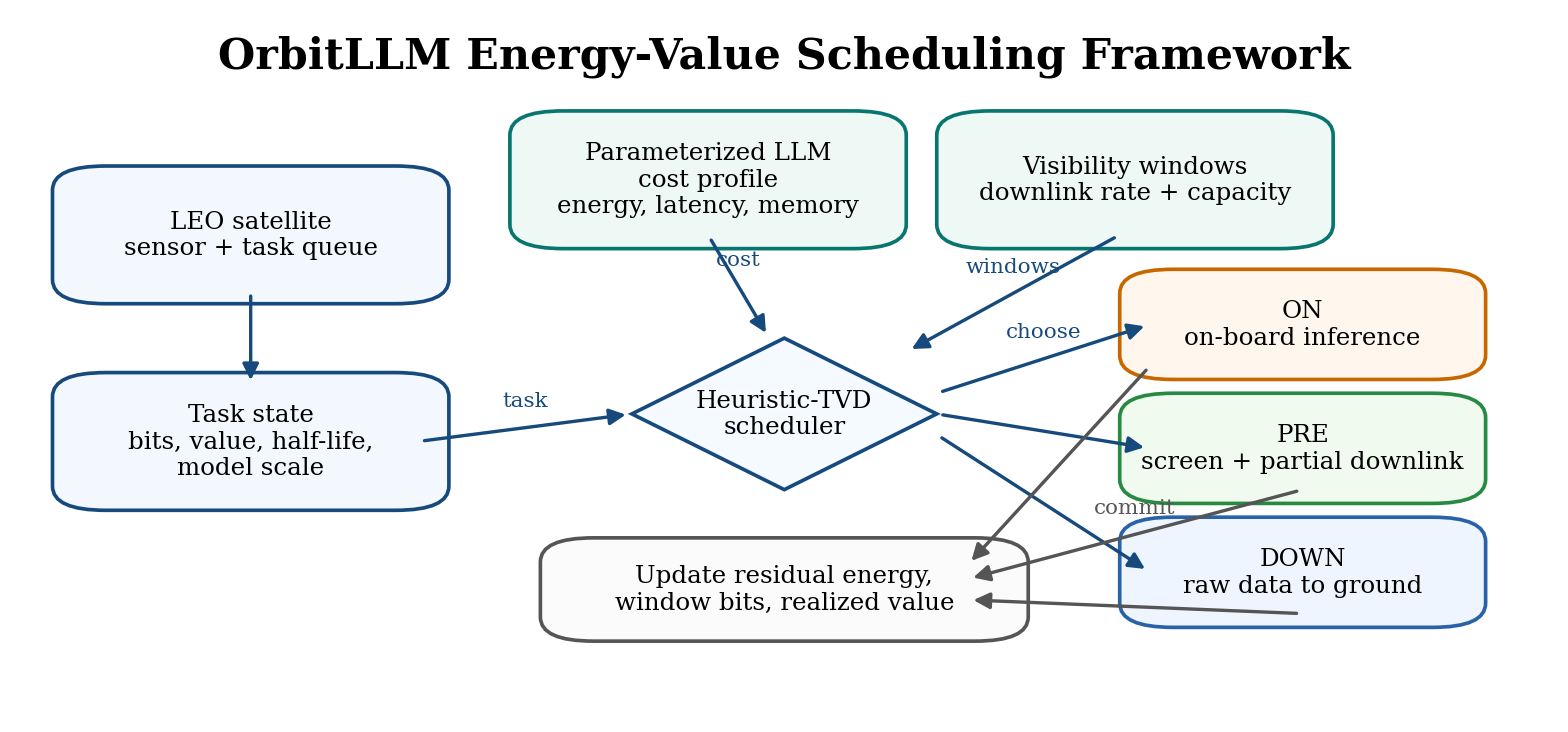
\includegraphics[width=\columnwidth]{figures/architecture.png}
  \caption{OrbitLLM architecture. A profile of LLM inference costs and a visibility-window timeline feed an online energy--value scheduler that chooses on-board inference, direct downlink, or pre-screening with partial downlink.}
  \label{fig:arch}
\end{figure}

\subsection{Visibility and Tasks}
The horizon is discretized into time slots $t=1,\ldots,T$ of duration $\Delta$. The orbital schedule gives a visibility indicator $v_t$ and rate $r_t$ when $v_t=1$. For a visibility window $w$, the available downlink capacity is
\begin{equation}
B_w=\sum_{t\in w} r_t\Delta .
\label{eq:bw}
\end{equation}
Task $i$ arrives at time $a_i$ and is described by $(d_i,s_i,V_i^0,\tau_i,n_i^p,n_i^d)$: raw bits, required model scale, immediate value, value half-life, prefill tokens, and decode tokens. If completed at time $c_i$, the realized value is
\begin{equation}
V_i(c_i)=V_i^0\exp\!\left(-\frac{c_i-a_i}{\tau_i}\right), \qquad c_i\ge a_i .
\label{eq:value}
\end{equation}
Small $\tau_i$ models time-critical observations such as wildfire onset; large $\tau_i$ models archival mapping.

\subsection{Actions and LLM Costs}
The scheduler chooses $x_i\in\{\textsc{on},\textsc{down},\textsc{pre}\}$. \textsc{on} runs the full model on board; \textsc{down} transmits raw data; \textsc{pre} is a lightweight semantic compression action inspired by value-aware data selection~\cite{denby2023kodan}. It can be implemented by an ROI selector, confidence-gated detector, or small encoder that emits metadata plus selected patches. We model it by a retained-bit ratio $\rho_i$ and a utility-retention factor $\eta_i$: it transmits $\rho_i d_i$ bits and realizes $\eta_i V_i(c_i)$. These parameters are not hidden constants; \Cref{sec:exp} sweeps them to show when PRE is useful. For model scale $s_i$, quantization $q$, and context $n_i^p+n_i^d$, the profile gives prefill energy $e^p$, decode energy $e^d$, throughput, and peak memory. Full on-board energy is
\begin{equation}
E_i^{\textsc{on}}=e^p_{s_i,q}n_i^p+e^d_{s_i,q}n_i^d .
\label{eq:eon}
\end{equation}
The pre-screen action uses a configurable fraction of this energy and memory and is evaluated across multiple $\rho_i,\eta_i$ regimes.

\subsection{Optimization Problem}
The objective is to maximize cumulative value subject to battery, downlink, and memory feasibility:
\begin{align}
\max_{\{x_i,\rho_i\}}\quad & \sum_i V_i(c_i(x_i)) \label{eq:obj}\\
\text{s.t.}\quad
& \sum_{i:x_i=\textsc{on}}E_i^{\textsc{on}}+\sum_{i:x_i=\textsc{pre}}E_i^{\textsc{pre}}\le E^{\max}, \label{eq:c-energy}\\
& \sum_{i\in w} b_i(x_i)\le B_w,\quad \forall w, \label{eq:c-bw}\\
& \mathrm{peakmem}(s_i,q,n_i^p+n_i^d)\le M^{\max}. \label{eq:c-mem}
\end{align}
Here $b_i(\textsc{down})=d_i$, $b_i(\textsc{pre})=\rho_i d_i$, and $b_i(\textsc{on})=0$; PRE values are multiplied by $\eta_i$. Even with known arrivals this contains a multiple-choice knapsack problem; the MILP in \Cref{sec:policy} is therefore an offline upper bound rather than an on-board algorithm.
